\subsection{A uniform continuation certificate}
This subsection proves Theorem~\ref{thm:paths-main}, including the connection of the successive zero discs.

\begin{lemma}[Uniform Rouch\'e test]\label{lem:rouche}
Let $F(s,a)$ be holomorphic in $s$ near the closed disc $|s-c|\le r$ and twice continuously differentiable in the real parameter interval $|a-a_0|\le h$, with the indicated mixed derivatives continuous. Suppose a complex number $b$ and nonnegative bounds satisfy
\[
\begin{gathered}
 |F(c,a_0)|\le\epsilon,\qquad |F_s(c,a_0)-b|\le\delta,\\
 |F_a(c,a)|\le T,\qquad |F_{sa}(c,a)|\le U,\qquad
 |F_{ss}(s,a)|\le M_2.
\end{gathered}
\]
If
\begin{equation}\label{eq:rouche}
 \epsilon+hT+r(\delta+hU)+\tfrac12M_2r^2<r|b|,
\end{equation}
then for every parameter in the interval the disc contains exactly one zero, counted with multiplicity. It is simple and varies continuously with the parameter.
\end{lemma}
\begin{proof}
At a fixed parameter, Taylor's formula along the straight segment from $c$ to $s$ gives
\[
 F(s,a)=F(c,a)+F_s(c,a)(s-c)
 +(s-c)^2\int_0^1(1-u)F_{ss}(c+u(s-c),a)\,du.
\]
The fundamental theorem of calculus in $a$ bounds the first term by $\epsilon+hT$ and bounds $|F_s(c,a)-b|$ by $\delta+hU$. On the circle the difference from $b(s-c)$ is therefore strictly smaller than $|b(s-c)|$. Rouch\'e's theorem gives one zero counted with multiplicity, so it is simple. The implicit-function theorem gives local continuous branches; uniqueness in the disc identifies them on overlaps and gives continuity on the entire interval.
\end{proof}

We now specify all analytic quantities used in the finite test. For integers $N,M\ge1$ put $A=N+a$ and
\begin{align*}
 G(s,a)={}&\sum_{n=0}^{N-1}(n+a)^{-s}
 +\frac{A^{1-s}}{s-1}+\frac12A^{-s}\\
 &+\sum_{k=1}^{M}\frac{B_{2k}}{(2k)!}
       (s)_{2k-1}A^{-s-2k+1}.
\end{align*}
Euler--Maclaurin summation gives $\zeta(s,a)=G(s,a)+R(s,a)$, with
\[
 R(s,a)=-\frac{(s)_{2M}}{(2M)!}
   \int_N^\infty \widetilde B_{2M}(x)(x+a)^{-s-2M}\,dx.
\]
Here $B_{2k}$ are Bernoulli numbers and $\widetilde B_{2M}$ is the periodic Bernoulli polynomial. This identity follows first for $\Re s>1$ and then by analytic continuation wherever $\Re s+2M>1$. Its convergence there is locally uniform, so the required differentiations under the integral are justified.

Write $P(s)=(s)_{2M}$, $B=\Re s+2M$, and suppose $A>1$, $B>1$. The bound
\[
 \frac{|\widetilde B_{2M}(x)|}{(2M)!}
 \le\frac{2\zeta(2M)}{(2\pi)^{2M}}
 <\frac4{(2\pi)^{2M}}
\]
comes from its Fourier series. With $v=(B-1)^{-1}$ define
\[
\begin{aligned}
 J_0&=A^{1-B}v,\\
 J_1&=J_0(\log A+v),\\
 J_2&=J_0((\log A)^2+2v\log A+2v^2).
\end{aligned}
\]
Integration by parts verifies $J_j=\int_A^\infty(\log u)^ju^{-B}\,du$ for $j=0,1,2$. Differentiating the remainder consequently gives the explicit bounds
\begin{align*}
 |R|&\le C_M|P|J_0,\\
 |R_s|&\le C_M(|P'|J_0+|P|J_1),\\
 |R_{ss}|&\le C_M(|P''|J_0+2|P'|J_1+|P|J_2),
 \qquad C_M=\frac4{(2\pi)^{2M}}.
\end{align*}
These are the real-positive-parameter specialization of the Euler--Maclaurin bounds in \citet{Johansson}. No asymptotic error estimate without an explicit bound is used.

For a test interval choose $b=G_s(c,a_0)$. The bounds just given enclose $\epsilon$, $\delta$, and $M_2$. The identities
\[
 F_a(c,a)=-c\zeta(c+1,a),\qquad
 F_{sa}(c,a)=-\zeta(c+1,a)-c\zeta_s(c+1,a)
\]
give $T$ and $U$ by one more Euler--Maclaurin evaluation. All finite sums and their first two $s$-derivatives are evaluated by the product rule, using
\[
 \partial_s^j x^{-s}=(-\log x)^jx^{-s},\qquad j=0,1,2.
\]
The disc is enclosed in its axis-parallel square when evaluating derivative bounds, which can enlarge the bounds but cannot invalidate them.

\begin{table}[htbp]
\centering\small
\begin{tabular}{r r r r r}
\toprule
$k$ & $\gamma_k$ & $\Re\rho_k(1)$ & $\Im\rho_k(1)$ & intervals\\
\midrule
1&14.134725141735&1.407788040653&23.327987754559&502\\
2&21.022039638772&0.410921753828&31.715410442191&512\\
3&25.010857580146&1.367688181122&38.419105560643&512\\
4&30.424876125860&0.594418197071&42.399454183542&512\\
5&32.935061587739&0.245270111140&48.772923691752&512\\
\bottomrule
\end{tabular}
\caption{The initial centres are $1/2+i\gamma_k$. Each initial and final displayed centre has a certified zero within radius $2\cdot10^{-12}$. The table does not claim that ordering by height is preserved among all zeros.}\label{tab:paths}
\end{table}

\begin{proof}[Proof of Theorem~\ref{thm:paths-main}]
Use $N=40$, $M=24$, and elementary interval arithmetic at 45 decimal digits of working precision. The Bernoulli coefficients are computed as exact rationals. Candidate centres are obtained at higher precision, then treated as decimal rational inputs; their numerical accuracy is not assumed by the certificate. The test of Lemma~\ref{lem:rouche} is performed with outward-rounded interval operations. In particular the upper enclosure of its left side must be strictly below the lower enclosure of its right side.

For each starting centre, a disc of radius $10^{-12}$ is tested at $a=1$. Begin parameter subdivision with intervals of length $1/64$ and bisect a failed interval. At each midpoint, a numerical candidate zero is chosen and enclosed in a disc whose radius is $1.3$ times the larger distance to the two endpoint candidates, plus $10^{-9}$. Those distances choose a candidate radius only; both endpoint inclusions are subsequently checked by interval inequalities. If the uniform Rouch\'e test or an inclusion fails, the parameter interval is bisected and tested again.

Every shared parameter endpoint is separately certified in a disc of radius $10^{-12}$. That disc is verified to lie strictly inside each adjacent uniform-test disc. Its one zero must therefore be the zero in both adjacent discs. This proves connection across every endpoint, instead of assuming that nearby numerical roots represent the same branch.

The five finite lists have respectively $502,512,512,512,512$ accepted intervals covering $[1,2]$ without gaps. The largest ratios of the two sides of \eqref{eq:rouche} are respectively less than
\[
 0.998,\quad0.873,\quad0.863,\quad0.935,\quad0.898.
\]
Thus every test is strict. The endpoint discs are contained in the radius-$2\cdot10^{-12}$ discs about the rounded values in Table~\ref{tab:paths}; these larger discs remain inside their uniform-test discs. This proves the endpoint assertions and uniqueness there.

The initial discs are disjoint. If two of the resulting simple-root branches met, their equality set would be closed by continuity and open by local implicit-function uniqueness. It would then be all of the connected interval, contradicting the disjoint initial discs. This proves distinctness. The two stated inequalities for real parts follow from the endpoint radii.

The accompanying programs \emph{Hurwitz interval continuation} and \emph{Hurwitz path figure} provide the verifier, finite interval lists, and plotted centres. The workbench record address is \url{\workbenchurl}. The certificate relies on elementary interval arithmetic and the displayed analytic bounds; it is not a proof-assistant formalization of the interval library.
\end{proof}

\begin{figure}[htbp]
\centering
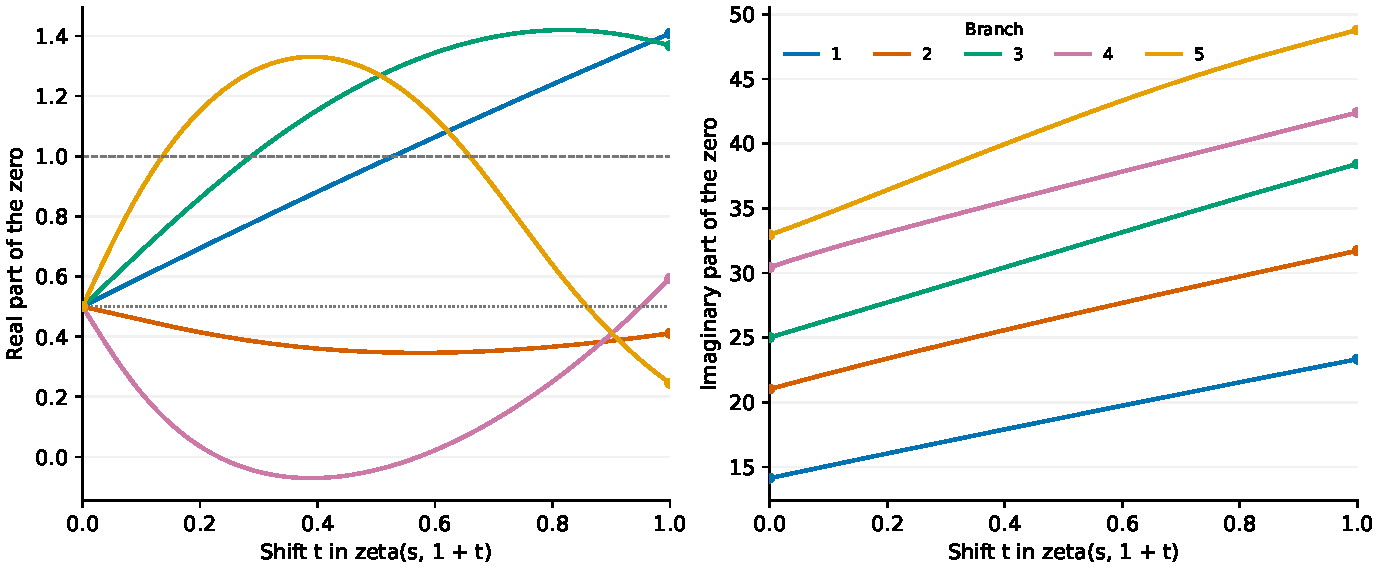
\includegraphics[width=\linewidth]{figures/hurwitz_paths.pdf}
\caption{The five certified branches as the first summand is removed. Curves join certified endpoint centres; the connecting segments are visual interpolation. The horizontal reference lines in the left panel are $\Re s=1/2$ and $\Re s=1$. Uniform disc certificates, rather than the drawn segments, prove continuation between the sampled points.}\label{fig:paths}
\end{figure}
